\chapter{工欲善其事,必先利其器}
\label{cha:pre-requisite}

用\LaTeX{}撰写毕业论文是一件赏心乐事,前提是你得会。网上关于\LaTeX{}的入门教程很多,下面这
几个就很不错,花一两天时间去熟悉一下,

\begin{enumerate}
\item \LaTeX{} on Wikibooks\footnote{\url{https://en.wikibooks.org/wiki/LaTeX}}
\item The very short guide to typesetting with
  \LaTeX{}\footnote{\url{http://tug.ctan.org/info/latex-veryshortguide/veryshortguide.pdf}}
\item The not so Short Introduction to
  \LaTeX{}\footnote{\url{https://www.ctan.org/tex-archive/info/lshort/english/?lang=en}}
\end{enumerate}
有了对\LaTeX{}的基础认识之后,再接着往下看。

\section{工作环境}
\label{sec:env}

工作环境当然要清静、优雅。一杯热咖啡,配上轻音乐……除此之外,你还需要一台电脑,最好是像我用
的电脑:

\begin{description}
\item[硬件:]不用太高级,但内存最好大一些,不少于4G为宜,因为在我看,CPU已经足够快了,电脑
  运行是否顺畅,更多的是取决于内存是否充足。
\item[操作系统:]Debian
  GNU/Linux\footnote{\url{https://en.wikipedia.org/wiki/Debian}}的测试(testing)版。为什么不用MS
  Windows\footnote{\url{https://en.wikipedia.org/wiki/Microsoft_Windows}}? 因为~\ldots 当
  然不是它不好,而是我缺乏足够的耐心。我的Debian系统从来不考验我的耐心。
\item[桌面环境:]不需要。有个window manager就足够了。我喜欢Sawfish window
  manager\footnote{\url{https://en.wikipedia.org/wiki/Sawfish_(window_manager)}},它界面足够
  的简单,功能足够的丰富,配置足够的容易。而且和Emacs一样,它也
  是用Lisp\footnote{\url{https://en.wikipedia.org/wiki/Lisp_(programming_language)}}写成的,
  算是Emacs\footnote{\url{https://en.wikipedia.org/wiki/Emacs}}的近亲吧。
  这是我偏爱Sawfish的一个重要原因。

  如果你有个大屏幕,那么可以试试%
  i3\footnote{\url{https://en.wikipedia.org/wiki/I3_(window_manager)}},%
  一个很不错的平铺式窗口管理器(tiling window %
  manager\footnote{\url{https://en.wikipedia.org/wiki/Tiling_window_manager}})。%
  它可以自动让所有的窗口互不重叠地铺满整个屏幕,非常适合大屏幕操作。%
  对于我14吋的小屏幕,还是Sawfish更友好些,因为它能方便地让我全屏操作。
  Sawfish和i3有个共同的优点,就是支持全键盘操作,有了这个,你可以完全忘掉鼠标的存在。
  
  除了窗口管理器,显然你还需要几个“窗口”。下面这三个恐怕是必须有的,

  \begin{description}
  \item[Web浏览器] 原来我用chromium\footnote{%
      \url{https://en.wikipedia.org/wiki/Chromium_(web_browser)}},2019年初开始,改
    用qutebrowser \footnote{%
      \url{https://en.wikipedia.org/wiki/Qutebrowser}} ,因为它小、快、灵、省内存、支持全键
    盘操作;
  \item[PDF阅读工具] 我用Emacs的pdf-tools插件。在Emacs里,可以在一个buffer里写tex,在另一
    个buffer里看PDF。还可以很方便地在两个buffer中对应的位置跳来跳去;
  \item[终端] 我用st\footnote{%
      \url{https://en.wikipedia.org/wiki/Suckless.org}}。其实,终端软件都差不多,有一个就
    行。真正不可或缺的是tmux\footnote{\url{https://en.wikipedia.org/wiki/Tmux}},有了它,
    一个终端可以当一万个用。
  \end{description}
\item[\LaTeX{}套件:] TeXLive\footnote{\url{https://en.wikipedia.org/wiki/TeX_Live}},它完备
  而庞大,但我们只需要其中很少的一些软件包就够了。附录\ref{app:pkg}中列出了参照本教程写论
  文所需的所有软件包,可供参考。
\item[中文字体:] 完全不必操心,因为TeXLive有很好的中文支持。如果抛开\TeX{}不谈,就日常使用而
  言,我比较喜欢Noto字体\footnote{\url{https://en.wikipedia.org/wiki/Noto_fonts}}。
  它是Google推出的开源字体。Debian库里自带,装上就好。所谓“Noto”就是No tofu的意思,也就是
  说Noto字体的终极目标是消灭所有的豆腐块(缺字)。Noto有专门的CJK字体包,只是尚缺楷体。%
  楷体我用Debian库里自带的arphic-ukai,它是台湾文鼎科技\footnote{%
    \url{https://en.wikipedia.org/wiki/Arphic_Technology}}推出的开源字体。
  你当然也可以选用Windows字体,只要从你的Windows系统里拷贝过来就行了。这也许是你人生中唯一需要Windows的时候。
\item[编辑器:]Emacs \(+\) \auctex\footnote{\url{https://en.wikipedia.org/wiki/AUCTeX}} \(+\)
  Yasnippet\footnote{\url{https://www.emacswiki.org/emacs/Yasnippet}} \(+\)
  pdf-tools\footnote{\url{https://github.com/politza/pdf-tools}}。
  \begin{itemize}
  \item Emacs是世界上最强大的编辑器\cite{emacs},没有之一。作为计科专业的学生,如果你不熟悉它的使用,
    怎么好意思写毕业论文呢?
  \item \auctex{}是一个历史悠久、功能强大的Emacs插件,它为我们编辑\LaTeX{}文件提供了丰富的快捷
    键操作\cite{auctex};
  \item Yasnippet也是Emacs的插件,它的功用就是为{\LKeyTab}键施加魔法\cite{yasnippet}。有了它,期
    待奇迹出现的时候,你只要左手小指在{\LKeyTab}键上轻轻一按……当然,你得先学会写魔咒(snippets)
    才行\,\Frowny{}。\label{p:yasnippet}放松,snippets都是很简单的小东西,去看看
    \texttt{\char`~/.emacs.d/snippets/latex-mode/}目录里的东西,我担保你能无师自通。
  \item pdf-tools,前面已经提过了。即使不写\TeX{},单纯地为了阅读PDF文件,pdf-tools也是目
    前我认为最好用的阅读器,因为除了阅读,还可以标注PDF。    
  \end{itemize}

  简而言之,有了上面几个插件,Emacs就成了一个强大的\LaTeX{}排版IDE\footnote{集成开发环境(Integrated
    Development Environment)。}(图~\ref{fig:screenshot})。有了它,写论文可以像领导说套话一样顺滑流畅。
\end{description}

\begin{figure}[ht]
  \centering
  \begin{center}
    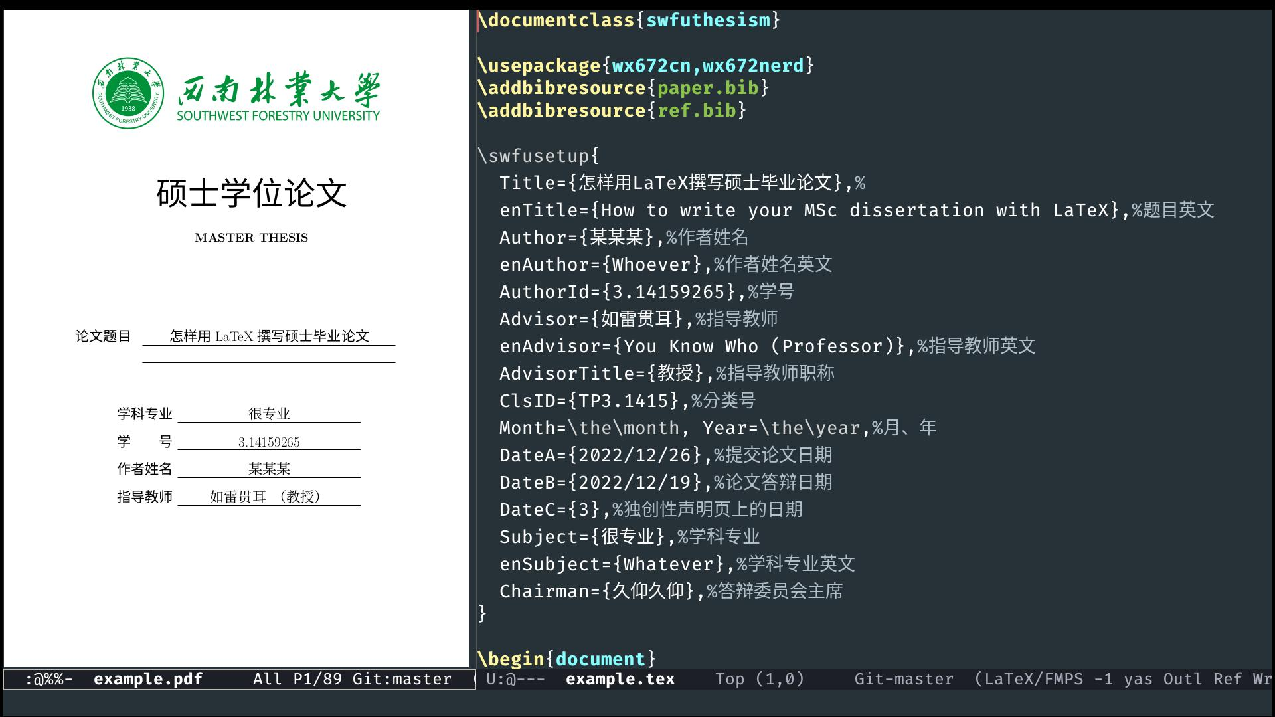
\includegraphics[width=.9\textwidth]{screenshot}
  \end{center}
  \caption{在Emacs中编辑、预览论文\label{fig:screenshot}}  
\end{figure}

附录\ref{app:pkg}中列出了我的Debian系统上安装的与写论文相关的所有软件包,当然,清单里的
东西并非都是必需。其实,除了中文字体之外,其它的一切,你都可以根据自己的偏好来选择。如果你
打算用英文写论文的话,那么连中文字体都可以省略了。不管怎么说,上面提到的都是我个人的偏好,
本教程也将以此为基础,逐步展开。

至于如何安装、配置好这样一个工作环境,如果你是本校的学生,那么当然可以直截找我帮忙。如果找不到我,那么你可以参考一下我曾经写过的一个比较潦草的%
\href{https://github.com/wx672/lecture-notes/blob/master/linux/tutorials/install/install.html}{《Debian安装指导》}\footnote{%
  \url{https://github.com/wx672/lecture-notes/blob/master/linux/tutorials/install/install.html}},也许有点过时,但应该还是能对你有点帮助的。

%%% Local Variables:
%%% mode: latex
%%% TeX-master: "../example"
%%% End:
